% REMEMBER: You must not plagiarise anything in your report. Be extremely careful.

\documentclass{l4proj}


%
% put any additional packages here
%

\begin{document}

%==============================================================================
% METADATA

\title{%
    \includesvg[width=200pt]{images/title_logo.svg}\par
    {\Huge Portion Mate \par}
    {\Large Daily Food Intake Tracker \par}
    \large
}
\author{Inesh Bose}
\date{Academic Session 2021-22}

\maketitle

%==============================================================================
% ABSTRACT

\begin{abstract}
    Every abstract follows a similar pattern. Motivate; set aims; describe work; explain results.
    \vskip 0.5em
    ``XYZ is bad. This project investigated ABC to determine if it was better.
    ABC used XXX and YYY to implement ZZZ. This is particularly interesting as XXX and YYY have
    never been used together. It was found that
    ABC was 20\% better than XYZ, though it caused rabies in half of subjects.''
\end{abstract}

%==============================================================================
% ACKNOWLEDGEMENTS

\begin{acknowledgements}
    I thank my supervisor Dr. Oana Andrei for her guidance. My previous / current employers who have given me experience and knowledge in my area of interest - computing and software development. The participants who helped evaluate the project and provide important feedback. Lastly, my friends and family.
\end{acknowledgements}

%==============================================================================
% EDUCATION REUSE CONSENT FORM
% If you consent to your project being shown to future students for educational purposes
% then insert your name and the date below to  sign the education use form that appears in the front of the document.
% You must explicitly give consent if you wish to do so.
% If you sign, your project may be included in the Hall of Fame if it scores particularly highly.
%
% Please note that you are under no obligation to sign
% this declaration, but doing so would help future students.
%

\def\consentname {Inesh Bose} % your full name
\def\consentdate {20 March 2022} % the date you agree
%
\educationalconsent

%==============================================================================

\tableofcontents

%==============================================================================
%% Notes on formatting
%==============================================================================
% The first page, abstract and table of contents are numbered using Roman numerals and are not
% included in the page count.
%
% From now on pages are numbered
% using Arabic numerals. Therefore, immediately after the first call to \chapter we need the call
% \pagenumbering{arabic} and this should be called once only in the document.
%
% Do not alter the bibliography style.
%
% The first Chapter should then be on page 1. You are allowed 40 pages for a 40 credit project and 30 pages for a
% 20 credit report. This includes everything numbered in Arabic numerals (excluding front matter) up
% to but excluding the appendices and bibliography.
%
% You must not alter text size (it is currently 10pt) or alter margins or spacing.
%
%
%=============================================================================
%
% IMPORTANT
% The chapter headings here are **suggestions**. You don't have to follow this model if
% it doesn't fit your project. Every project should have an introduction and conclusion,
% however.
%
%=============================================================================


%=============================================================================
% INTRODUCTION
% Why should the reader care about what are you doing and what are you actually doing?
% **Motivate** first, then state the general problem clearly.

% ## Guidance

% ### Who is the reader?

% This is the key question for any writing. Your reader:

% -   is a trained computer scientist: *don’t explain basics*.

% -   has limited time: *keep on topic*.

% -   has no idea why anyone would want to do this: *motivate clearly*

% -   might not know *anything* about your project in particular: *explain
%     your project*.

% -   but might know precise details and check them: *be precise and
%     strive for accuracy.*

% -   doesn’t know or care about you: *personal discussions are
%     irrelevant*.

% Remember, you will be marked by your supervisor and one or more members
% of staff. You might also have your project read by a prize-awarding
% committee or possibly a future employer. Bear that in mind.

% ### References and style guides

% There are many style guides on good English writing. You don’t need to
% read these, but they will improve how you write.

% -   *How to write a great research paper* (**recommended**, even though
%     you aren’t writing a research paper)

% -   *How to Write with Style* . Short and easy to read. Available
%     online.

% -   *Style: The Basics of Clarity and Grace* A very popular modern
%     English style guide.

% -   *Politics and the English Language* A famous essay on effective,
%     clear writing in English.

% -   *The Elements of Style* Outdated, and American, but a classic.

% -   *The Sense of Style* Excellent, though quite in-depth.

% #### Citation styles

% -   If you are referring to a reference as a noun, then cite it as: “
%     discusses the role of language in political thought.”

% -   If you are referring implicitly to references, use: “There are many
%     good books on writing .”

% There is a complete guide on good citation practice by Peter Coxhead
% available here: <http://www.cs.bham.ac.uk/~pxc/refs/index.html>. If you
% are unsure about how to cite online sources, please see this guide:
% <https://student.unsw.edu.au/how-do-i-cite-electronic-sources>.

% ### Plagiarism warning

% <div class="highlight_title">

% WARNING

% If you include material from other sources without full and correct
% attribution, you are commiting plagiarism. The penalties for plagiarism
% are severe. Quote any included text and cite it correctly. Cite all
% images, figures, etc. clearly in the caption of the figure.

% </div>

\chapter{Introduction}

% reset page numbering. Don't remove this!
\pagenumbering{arabic}

\section{Overview}

In this dissertation, we discuss the development and evaluation strategies adopted for a cross-platform application named "Portion Mate". This project was proposed by Dr. Oana Andrei for the Level 4 Individual Project course [https://www.gla.ac.uk/coursecatalogue/course/?code=COMPSCI4025P] at the University of Glasgow during the academic year 2021-22, and undertaken by student Inesh Bose.

\section{Motivation}

Mobile applications have been on the rise and demand ever since affordable smartphones were introduced with internet connections all over the globe. Since the devices are portable and small, the applications make accessing a service convenient and easy. [Put statistics and sources]

Fitness and food tracking applications exist, however most have not provided a very suitable way of logging activity therefore becoming a burden on users. Food, despite being a very cultural and social element in many lifestyles and regions, should be monitored and consumed with diet in mind.

\section{Aims}

As a product-focused software engineering project, our goal is to \textbf{make a maintainable, efficient, robust and reliable system}. The end-users are first in mind, however, developers are second so that understanding and working on the codebase is easy.

\section{Outline}

This dissertation is structured into seven chapters:

\begin{itemize}
    \item \textbf{Chapter 2} \textit{Background} shares the underlying circumstances and work already done related to the area of the project - diet and nutrition
    \item \textbf{Chapter 3} \textit{Requirements} discusses the expectations and plan for the output
    \item \textbf{Chapter 4} \textit{Design} conveys solutions for the problems the project plans to solve, and any that may come up during the implementation
    \item \textbf{Chapter 5} \textit{Implementation} is about putting everything planned into practice and creating the final product with technical discussion
    \item \textbf{Chapter 6} \textit{Evaluation} evaluates the final implemented product by discussing methods and analysis conducted
    \item \textbf{Chapter 7} \textit{Conclusion} summarises and looks back on the dissertation sharing lessons that were learnt, future work and projects that were inspired by this.
\end{itemize}


%=============================================================================
% BACKGROUND
% What did other people do, and how is it relevant to what you want to do?

% ## Guidance

% -   Don’t give a laundry list of references.

% -   Tie everything you say to your problem.

% -   Present an argument.

% -   Think critically; weigh up the contribution of the background and
%     put it in context.

% -   **Don’t write a tutorial**; provide background and cite references
%     for further information.

\chapter{Background}

Talk about related apps, what features inspired, why not use them instead..

\section{Eating Habits in the UK}

The eating lifestyle in the UK is to have three main meals a day - Breakfast (between 7:00 and 9:00), Lunch (between 12:00 and 14:00), and Dinner or "Tea" (between 18:00 and 20:00).

It is not fair to generalise meals as they vary a lot, the "traditional English breakfast" is known to be a plate with fried eggs, bacon, sausages, baked beans, black pudding and toast. Lunch is simple and easy consisting of sandwiches (also known as "butty") that can have many different items between the bread, the most common being ham and cheese. In the current times, the nation also feeds on meal deals offered by chains like Greggs and Tesco. The rule followed for dinner is "meat and two veg" and typically that is a roast dinner.

A study also discovered that many people in the UK have not cooked a meal in years, but resort to processed food such as frozen pizzas that only need to be prepared in the oven for 10 minutes. [paper required]

While some cultures restrict meat, some view meat as a social celebration, a Reddit post discussed the consumption of meat in the UK [citation] and most answers justify the meat for the protein and adding taste to relatively "boring" dinners that would otherwise consist of vegetables only. Unfortunately, this causes a big impact on the environment since meat production creates a large percentage (60\%) of greenhouse gases every year.

A new trend has also been on the rise due to this called "veganism" where individuals would choose to cut out all animals product (such as dairy and poultry) from their diet. So, many products and companies have started creating alternatives.

Students usually do not have their diet as a priority.... more needed

\subsection{Day Plan}

\subsection{Processed Foods}

\subsection{Diets}

Veganism statistics, etc. Students here as well.

\section{Eatwell Guide}

The National Health Service (NHS) is a unified publicly funded healthcare system in the United Kingdom. Given the eating habits in the country, the NHS suggests a guide that encourages people to "eat well" by showing how many portions of each food group should be consumed for a healthy, balanced diet. The guide is as follows:

\begin{itemize}
    \item at least 5 portions of \textbf{fruits and vegetables}
    \item meals based on \textbf{starchy carbohydrates} (such as potatoes, bread, rice and pasta) % choosing wholegrain versions where possible
    \item some \textbf{dairy} (or alternatives) consumption is important for calcium % protein and vitamins
    \item \textbf{protein} (from meat, beans, pulses and fish) should be about 2 portions % avoiding red and processed meat
    \item essential levels of \textbf{oils and fats}
    \item hydration should be aimed through having 6-8 glasses of \textbf{fluid} every day
    \item foods high in \textbf{sugar} are not needed, but if included, should be in small amounts
\end{itemize}

\subsection{Fruits \& Vegetables}

\subsection{Carbohydrates}

\subsection{Dairy}

\subsection{Protein}

\subsection{Oils \& Fats}

\subsection{Fluids}

\subsection{Sugars}

\section{Seeing a Professional}

% conversation with a dietitian

Eatwell Guide is generalised, but a professional gives targeted, tailored plan - compare

An expert who can provide guidance and prescriptions on eating habits is a \textbf{dietitian}. This may be confused with a nutritionist - the difference is that a dietitian is licensed and receive the title based on a classification by the World Health Organization [citation]. When seeking professional guide, there are likely to be follow ups, and accurate information is essential.

\section{The Client}

This project has been proposed by Dr. Oana M. Andrei - a lecturer at the University of Glasgow - who has been logging her portion intake on papers. [insert images]

\section*{Summary}

%=============================================================================
% REQUIREMENTS
% What is the problem that you want to solve, and how did you arrive at it?

% ## Guidance

% Make it clear how you derived the constrained form of your problem via a clear and logical process.

\chapter{Requirements}

\href{https://github.com/ineshbose/portion-mate/wiki/Requirements}{https://github.com/ineshbose/portion-mate/wiki/Requirements}

\section{Planning}

As instructed by Dr. Andrei, the project timeline was laid out through six blocks:

\begin{table}[h]
\begin{tabular}{llll}
\textbf{Block 1} & Weeks 1-4   & 27 Sep - 18 Oct & Planning Period                                 \\
\textbf{Block 2} & Weeks 5-13  & 25 Oct - 20 Dec & Setup Period                                    \\
\textbf{Block 3} & Weeks 14-15 & 27 Dec - 3 Jan  & Development Period                              \\
\textbf{Block 4} & Weeks 16-19 & 10 Jan - 31 Jan & (integrated with Block 3) \\
\textbf{Block 5} & Weeks 20-23 & 7 Feb - 28 Feb  & Deployment Period                               \\
\textbf{Block 6} & Weeks 24-26 & 7 Mar - 21 Mar  & Evaluation \& Writing Period                   
\end{tabular}
\end{table}

The backlog including tasks \& issues would be distributed and worked on using these blocks.

\section{Prioritisation}

Based on the block an issue is assigned to, the priority would also be estimated using the MoSCoW method that stands for "Must have, Could have, Should have, and Would be nice to have".

\section{User Requirements}

\section{System Requirements}

developer convenience

\subsection{Functional}

\subsection{Non-Functional}

\section*{Summary}

%=============================================================================
% DESIGN
% How is this problem to be approached, without reference to specific implementation details?

% ## Guidance

% Design should cover the abstract design in such a way that someone else might be able to do what you did, but with a different language or library or tool.

\chapter{Design}

\section{Considerations}

\subsection{Compatibility}

\subsection{Modularity}

\subsection{Reliability}

\subsection{Reusability}

\section{Software Architecture}

[object oriented]

\subsection{Model View Controller}

[also include ER diagram]

\subsection{Representational State Transfer}

\subsection{Plug-ins}

\section{Interface Design}

\subsection{Consistency}

\subsection{Accessibility}

\subsection{Customisation}

\subsection{Responsiveness}

\section*{Summary}

%=============================================================================
% IMPLEMENTATION
% What did you do to implement this idea, and what technical achievements did you make?

% ## Guidance

% You can't talk about everything. Cover the high level first, then cover important, relevant or impressive details.

\chapter{Implementation}

\section{Version Control}

Using version control was an important criteria for this dissertation. Despite being required, development would not have gone forward without it since it enables history, rollback, branching, and lot more allowing software development to be lot more flexible and less scary with many possibilities.

\subsection{Git \& GitHub}

There are different version control architectures (such as local, centralized), but Git is the most popular version control system system and uses a distributed repository architecture providing lots of advantages over other systems like resolving conflicts, easier branching and better performance overall.

[include diagram]

The remote repository is hosted on GitHub, which is equally popular as Git and owned by Microsoft. The service provides additional features for repositories on their platform like issue tracking, continuous integration and wikis [citation]. The project has taken every advantage of all features, and has also developed extensions to make the process extremely streamline (more in side projects [chapter] and automation [chapter]).

\subsection{Issue Branching}

Issue tracking systems, being industry standard, this project made sure to work with this strategy in the best possible way. This is also heavily inspired by Atlassian products - Jira and Bitbucket - that integrate to provide issues and branching mechanism. Exposure to this system was received during an internship at New Verve Consulting [link] in summer 2021. Pipelines were setup to enable the integration and automation (more discussed in [chapter]). Therefore, all implementations were done through issues and in different branches.

[branch graph, issues and PR examples]

\subsection{Hooks}

https://git-scm.com/book/en/v2/Customizing-Git-Git-Hooks

https://github.com/ineshbose/portion-mate/issues/52

Version control systems usually provide signals (hooks) when specific commands are run. With Git, a \code{pre-commit} hook has been setup that runs the code linters (mentioned in [chapter]) before the changes can be pushed onto the remote repository. The scripts that would run on these hooks could be setup using different packages like \code{pre-commit/pre-commit} [repo] and \code{typicode/husky} [repo] - the latter being the most popular. However, husky has drawbacks such as creating additional configuration files and running an install script which may create inconsistencies for developer environments; these were not required in version 4 of the package (currently on v7 at time of writing), but the project strongly prefers packages at their latest versions, an alternate \code{yyx990803/yorkie} was found (based on version 4 of husky, developed by the creator of Vue framework) that allows configuration to be in the \code{package.json} and not require installation of the script, but the package itself.

\begin{lstlisting}[language=json,caption={\href{https://github.com/ineshbose/portion-mate/blob/c51ee3f32d05df641157467169e9659732202b7b/package.json\#L22}{\code{./package.json}}}]
  "gitHooks": {
    "pre-commit": "npx lint-staged"
  }
\end{lstlisting}

\section{Environment setup}

As the foundation of the application, the development environment had to be configured keeping the requirements and future steps in mind. The major decision was with the languages that the stack will use that would require their compilers / interpreters.

\subsection{Python}

\subsubsection{Dependency Management}

Python3 includes the \code{pip} package management system that sources packages from the Python Package Index (PyPI). This package manager, however, requires manual configuration, like maintaing a virtual environment, updating the list of dependencies, and resolving peer-dependency version conflicts.

\begin{lstlisting}[language=bash, caption={\code{pip} usage example}]
  $ pip install -r requirements.txt
  $ pip install requests
  $ pip freeze > requirements.txt
\end{lstlisting}

https://github.com/ineshbose/portion-mate/pull/69

These issues have been addressed and resolved by Poetry [link] that maintains the dependencies in \code{pyproject.toml} and provide ways to make the project compatible like switching Python version easily and listing dependencies in a global way. Another similar solution is Pipenv that has some different pros and cons, but the development of Poetry is promising with the support of plugins in release version 1.12.

\subsubsection{Code formatting}

Python offers many different ways to write the same code, and personally, list comprehensions and inline conditions (one-liners) seem impressive, but they could make the one line of code very long. To ensure that code remains consistent and readable, \textit{Black} is a formatting tool that works in compliance with PEP8 [https://peps.python.org/pep-0008/] and also produces small diffs to make code reviews faster - useful for the development strategy.

\subsection{TypeScript}

\begin{lstlisting}[language=typescript, caption={type definition for creation object in \href{https://github.com/ineshbose/portion-mate/blob/c51ee3f32d05df641157467169e9659732202b7b/src/app/types/api.ts\#L28}{\code{./src/app/types/api.ts}}}]
export type CreateData<
  T extends GenericModel | ModelID = GenericModel,
  R extends keyof T | string = 'name'
> = Partial<Omit<T, 'id' | R>> & {
  [P in R]: R extends keyof T
    ? NonNullable<T[R]> extends GenericModel | ModelID
      ? CreateData<NonNullable<T[R]>> | ModelID
      : T[R]
    : any;
};
\end{lstlisting}

\subsubsection{Dependency Management}

The default package manager for Node.js is \code{npm} and it lists and updates dependencies in \code{package.json} automatically. In 2016, Facebook developed an alternative dubbed "Yet Another Resource Negotiator" popularly known as Yarn which provides better speed and stability than \code{npm}. Because of this, the package manager started to be preferred by many in the community. A few years later, the development for Yarn switched to a different team therefore releasing a rewrite called "Berry", keeping version 1 as "Classic". Yarn Berry changed the traditional approach of resolving dependencies through a feature called "Plug'n'Play". [discuss more about advantages and the paper on this feature] At the time of writing, the latest version of Yarn is 3.2.0. Since the approach for modern Yarn is unconventional, the project stuck to classic.

https://github.com/ineshbose/portion-mate/issues/44
https://github.com/ineshbose/portion-mate/pull/83

Additionally, Yarn also has a "workspaces" feature that allows the repository to use the monorepo strategy [more on this].

https://github.com/ineshbose/portion-mate/issues/71

\subsubsection{Code styling}

The majority of the codebase is expected to be TypeScript (which also enforces style rules onto JavaScript for type definitions) that would include React syntax (file extension \code{.[jt]sx}). All TypeScript code would be analysed using ESLint that supports ECMAScript standards to standardise and encourage compatibility. It is the most commonly used JavaScript linter, being downloaded over 14,000,000 times per week [citation]. As mentioned, since the code is not vanilla JavaScript, additional configurations had to be added to ESLint.

\begin{itemize}
    \item Prettier is an opinionated formatter (similar to \textit{Black} for Python [chapter]) and extends the formatting rules in ESLint
    \item React plugin for ESLint provides React specific linting rules
    \item TypeScript plugin enables ESLint to analyse \code{.tsx?} files
    \item Airbnb provides a JavaScript Style Guide [link] which is community preferred and can be setup along with ESLint
\end{itemize}

Note: file extensions written are in RegEx.

\subsection{Stack Specific}

\subsubsection{ngrok}

Since the application needs to be tested on mobile devices while running locally, the API calls are normally made to \code{localhost} which would not work on different devices. Therefore, the project uses a very unique, automated setup with ngrok making testing incredibly easy.

\begin{lstlisting}[language=javascript, caption={Automatic ngrok connection in \href{https://github.com/ineshbose/portion-mate/blob/c51ee3f32d05df641157467169e9659732202b7b/src/set-env.js\#L26}{\code{./src/set-env.js}}}]
const start = (file = `${__dirname}/.env`) => {
  const env = dotenv.parse(fs.readFileSync(file, 'utf-8'));
  const port = getPort(env.API_BASE);
  if (env.DEBUG.toLowerCase() === 'true' && port) {
    ngrok.connect(port).then((value) => {
      env.API_BASE = `${value}${env.API_BASE.split(`${port}`)[1]}`;
      writeToFile(env);
    });
  } else {
    writeToFile(env);
  }
};
\end{lstlisting}

\section{Technologies}

\subsection{Django server}

The backend server of Portion Mate was developed using the Django framework, written in Python, which follows the MVC architecture pattern described in [chapter]. The principle of this framework is \textbf{don't repeat yourself}. The framework advertises with "Batteries included" which means that it comes out of the box with libraries and utilities that could potentially be required for the development of the server, like authentication system and database connection. This could also be a downside for Django, since it makes the package bigger with modules that may be required; in that case, Flask [link] is an alternative. For this project, however, Django was a suitable choice.

\subsubsection{REST Framework}

As discussed in [chapter: rest architecture], the project would use a different technology for the frontend application, therefore to build a Web API, Django REST Framework was adopted. It provides with utilities like serializers, authentication policies and a browsable API that would help visualisation JSON data.

\subsubsection{OAuth}

\textbf{O}pen \textbf{Auth}orization is an access delegation mechanism used by many major companies for their applications. Users would need to access their information such as logs, these would be provided by this method. Since the project uses API calls between the Django server and the React application, the access occurs through token (but not to be confused with JWT mechanism), which would be given on login and have an expiry.

\begin{lstlisting}[language=json, caption={Access token example}]
{
    "access_token": "<your_access_token>",
    "token_type": "Bearer",
    "expires_in": 36000,
    "refresh_token": "<your_refresh_token>",
    "scope": "read write groups"
}
\end{lstlisting}

In HTTP requests, the token is added in the header as \code{Authorization}.

\subsubsection{GraphQL}

(Work in progress, may not be added)
In addition to the REST architecture, Portion Mate also has a setup for a new alternative query language for its API.

\subsection{React Native app}

The principle of this framework is \textbf{Learn once, write anywhere} - that translates to \textit{don't repeat yourself} in writing code, programs and applications in different languages / technologies to support native applications. Instead, React Native aims to use one codebase to support multiple platforms.

\subsubsection{Expo}

While React Native allows development of applications using React, there would be places where native development could be essential (like creating a \code{build.gradle} to publish on Android). However, Expo removes the need for all of that and would automatically build and bundle applications for cross-platform development.

\subsubsection{Axios}

Since the frontend application needs to make API requests to the server, axios client was used since it automates many elements that \code{fetch} (default HTTP client) fails to do (like transforming JSON data). It supports usage of Promises [more on this?] and more versions of browsers than \code{fetch} for compatibility.

The application uses and provides a consistent, uniform and easy integrated usage of axios by using a created instance that would keep user's \code{Authorization} header (along with an attached interceptor for refreshing / revoking token) and methods that reduce code repetition / duplication. (as reported by Code Climate)

\begin{lstlisting}[language=typescript, caption={created axios instance in \href{https://github.com/ineshbose/portion-mate/blob/c51ee3f32d05df641157467169e9659732202b7b/src/app/api/index.ts\#L20}{./src/app/api/index.ts}}]
export const axiosInstance = axios.create({
  baseURL: API_BASE,
});
\end{lstlisting}

\subsubsection{Eva Design System (UI Kitten)}

The user interface becomes the most important aspect of the application. Most code written deals with components and interface layout. Styling libraries provide methods to make design and development easier, for example Bootstrap is one of the most popular frontend frameworks that provides CSS classes like \code{navbar}, \code{float-start} and \code{bg-primary} that would set and style elements accordingly (as the class names would suggest).

\begin{lstlisting}[language=html, caption={example of a Card element as \href{https://getbootstrap.com/docs/5.1/components/card/\#example}{documented on Bootstrap v5}}]
<div class="card" style="width: 18rem;">
  <img src="..." class="card-img-top">
  <div class="card-body">
    <h5 class="card-title">Card title</h5>
    <p class="card-text">Some quick example text to build on the card title and make up the bulk of the card's content.</p>
    <a href="#" class="btn btn-primary">Go somewhere</a>
  </div>
</div>
\end{lstlisting}

For component-based frameworks like React and Vue, such libraries also get extended to provide additional functionality. In this example, Bootstrap would have React-Bootstrap (for React) and BootstrapVue (for Vue) [links] where, instead of using classes, components are predefined with lots of configuration options.

\begin{figure}
    \centering
    \noindent\begin{subfigure}{.49\textwidth}
    \begin{lstlisting}[language=html, caption={\href{https://react-bootstrap.github.io/components/cards/\#basic-example}{documented on React-Bootstrap}}]
    <Card style={{ width: '18rem' }}>
      <Card.Img variant="top" src="..." />
      <Card.Body>
        <Card.Title>Card Title</Card.Title>
        <Card.Text>
          Some quick example text to build
          on the card title and make up the
          bulk of the card's content.
        </Card.Text>
        <Button variant="primary">
            Go somewhere
        </Button>
      </Card.Body>
    </Card>
    \end{lstlisting}
    \end{subfigure}\hfill
    \begin{subfigure}{.49\textwidth}
    \begin{lstlisting}[language=html, caption={\href{https://bootstrap-vue.org/docs/components/card\#overview}{documented on BootstrapVue}}]
    <b-card
      title="Card Title"
      img-src="..."
      img-top
    >
      <b-card-text>
        Some quick example text to build on
        the card title and make up the bulk
        of the card's content.
      </b-card-text>
      <b-button href="#" variant="primary">
        Go somewhere
      </b-button>
    </b-card>
    \end{lstlisting}
    \end{subfigure}
    \caption{examples of Card components}
\end{figure}

Unfortunately, this does not translate for React Native, since most of the utilities have been made possible through CSS classes and mobile development does not use HTML or CSS [https://reactnative.dev/docs/style]. There are limited components available for native development, like View, Text and Image, and these can only be styled using certain allowed properties, like margins, border and flex (similar to CSS but not the same). This would pose lots of difficulties in the interface development. Fortunately, Akveo provides a library UI Kitten with native components styled according to the Eva Design System, yielding easy development and consistent interface. The design was adopted in the middle of development [issue https://github.com/ineshbose/portion-mate/issues/93]. However, at certain points, extra custom styling had to be added and that also seemed to be repetitive, whereas Bootstrap has a simple class mechanism. Inline styling is not good practice, and for React Native also causes performance issues. Therefore, a React Native equivalent for Bootstrap was developed so that components can take advantage of the defined "classes" [https://github.com/ineshbose/portion-mate/issues/116, https://github.com/ineshbose/portion-mate/pull/120/files].

\begin{lstlisting}[language=typescript, caption={root definition of App, using Eva Design and UI Kitten components in \href{https://github.com/ineshbose/portion-mate/blob/c51ee3f32d05df641157467169e9659732202b7b/src/app/App.tsx\#L28}{\code{./src/App.tsx}}}]
import { mapping, light, dark } from '@eva-design/eva';
import {
  ApplicationProvider,
  Button,
  ButtonProps,
  Icon,
  IconRegistry,
} from '@ui-kitten/components';
import { MaterialIconsPack } from './app/components/AppIcons';
import { ColorScheme } from './app/types';
import { ThemeContext } from './app/contexts/ThemeContext';
import Navigation from './app/navigation';
import { default as colors } from './app/assets/theme.json';
import { default as customMapping } from './app/assets/mapping.json';

export default function App() {
  // ...
  return (
    <>
      <IconRegistry icons={MaterialIconsPack} />
      <ThemeContext.Provider
        value={{ theme, setTheme, switchTheme, ThemeToggle }}
      >
        <ApplicationProvider
          mapping={mapping}
          customMapping={customMapping}
          theme={{ ...(isLightTheme ? light : dark), ...colors }}
        >
          <Navigation />
        </ApplicationProvider>
      </ThemeContext.Provider>
    </>
  );
}
\end{lstlisting}

\begin{lstlisting}[language=typescript, caption={custom style function in \href{https://github.com/ineshbose/portion-mate/blob/c51ee3f32d05df641157467169e9659732202b7b/src/app/constants/Styles/index.ts\#L28}{\code{./src/app/constants/Styles/index.ts}}}]
const PROVIDED_STYLES = <GlobalStyleSheet>{
  ...spacingStyles,
  ...displayStyles,
  ...flexStyles,
};

export default function createStyle<
  T extends StyleSheet.NamedStyles<T> | StyleSheet.NamedStyles<any>
>(styles: T | StyleSheet.NamedStyles<T>) {
  return StyleSheet.create({ ...PROVIDED_STYLES, ...styles });
}
\end{lstlisting}

\begin{figure}
    \centering
    \noindent\begin{subfigure}{.49\textwidth}
    \begin{lstlisting}[language=html, caption={using inline styles}]
    <div style="display: flex;">
      <div
        style="
          display: flex;
          align-items: 'center';
          justify-content: 'center';
          padding: 2;
        "
      >
        <!-- Spinner CSS is complex -->
        <div style="..."></div>

        <h3>Loading</h3>
      </div>
    </div>
    \end{lstlisting}
    \end{subfigure}\hfill
    \begin{subfigure}{.49\textwidth}

    \begin{lstlisting}[language=html, caption={using Bootstrap classes}]
    <div class="d-flex">
      <div
        class="
          d-flex
          align-items-center
          justify-content-center
          p-2
        "
      >
        <div class="spinner-border"></div>
        <p class="fs-3">
          Loading...
        </p>
      </div>
    </div>
    \end{lstlisting}
    \end{subfigure}
    \caption{plain HTML example, showing effect of Bootstrap}
\end{figure}

\begin{figure}
    \centering
    \noindent\begin{subfigure}{.49\textwidth}
    \begin{lstlisting}[language=html, caption={normal usage, with increased complexity [rnstyle]}]
    <SafeAreaView style={{ flex: 1 }}>
      <Layout
        style={{
          flex: 1,
          alignItems: 'center',
          justifyContent: 'center',
          padding: 2,
        }}
      >
        <Spinner size="giant" />
        <Text style={styles.title}>
          {'Loading...'}
        </Text>
      </Layout>
    </SafeAreaView>
    \end{lstlisting}
    \end{subfigure}\hfill
    \begin{subfigure}{.49\textwidth}

    \begin{lstlisting}[language=html, caption={example of usage like Bootstrap in \href{https://github.com/ineshbose/portion-mate/blob/82a726e58c501ab2b4fe9c5f18ac399fb29b0422/src/app/navigation/RootNavigator.tsx\#L13}{\code{src/app/navigation/RootNavigator.tsx}}}]
    <SafeAreaView style={styles.flex1}>
      <Layout
        style={[
          styles.flex1,
          styles.alignItemsCenter,
          styles.justifyContentCenter,
          styles.padding2,
        ]}
      >
        <Spinner size="giant" />
        <Text style={styles.title}>
          {'Loading...'}
        </Text>
      </Layout>
    </SafeAreaView>
    \end{lstlisting}
    \end{subfigure}
    \caption{React \textbf{Native} code; note - React Native does not allow \code{display: 'flex'} (CSS)}
\end{figure}

\subsection{Automation}

It is highly desirable and preferred to have many processes automated. As discussed in [version control chapter], pipelines and hooks were taken advantage of.

\subsubsection{Pipelines}

[diagram of all workflows]

\subsubsection{Services}

Code Climate, Codacy, Read the docs, Overleaf

\section{Challenges}

Mentioned in eva design system

Setup of repo and workflows

Learning curve with React Native

\section*{Summary}

%=============================================================================
% EVALUATION
% How good is your solution? How well did you solve the general problem, and what evidence do you have to support that?

% ## Guidance

% -   Ask specific questions that address the general problem.

% -   Answer them with precise evidence (graphs, numbers, statistical
%     analysis, qualitative analysis).

% -   Be fair and be scientific.

% -   The key thing is to show that you know how to evaluate your work,
%     not that your work is the most amazing product ever.

% ## Evidence

% Make sure you present your evidence well. Use appropriate
% visualisations, reporting techniques and statistical analysis, as
% appropriate.

% If you visualise, follow the basic rules, as illustrated in Figure
% [\[fig:boxplot\]][1]:

% -   Label everything correctly (axis, title, units).

% -   Caption thoroughly.

% -   Reference in text.

% -   **Include appropriate display of uncertainty (e.g. error bars, Box
%     plot)**

% -   Minimize clutter.

% See the file `guide_to_visualising.pdf` for further information and
% guidance.

%   [1]: #fig:boxplot

\chapter{Evaluation}

\section{Testing}

% app itself, being established and fulfilling requirements

\section{Survey Design}

How were the questions thought of and formed?

\subsection{Demographics}

Why need demographics?

\subsection{Effect}

Measuring effect

\section{System Usability Survey}

Neutral linear scale, inverted questions.

\section{Results}

% \begin{figure}
%     \centering
%     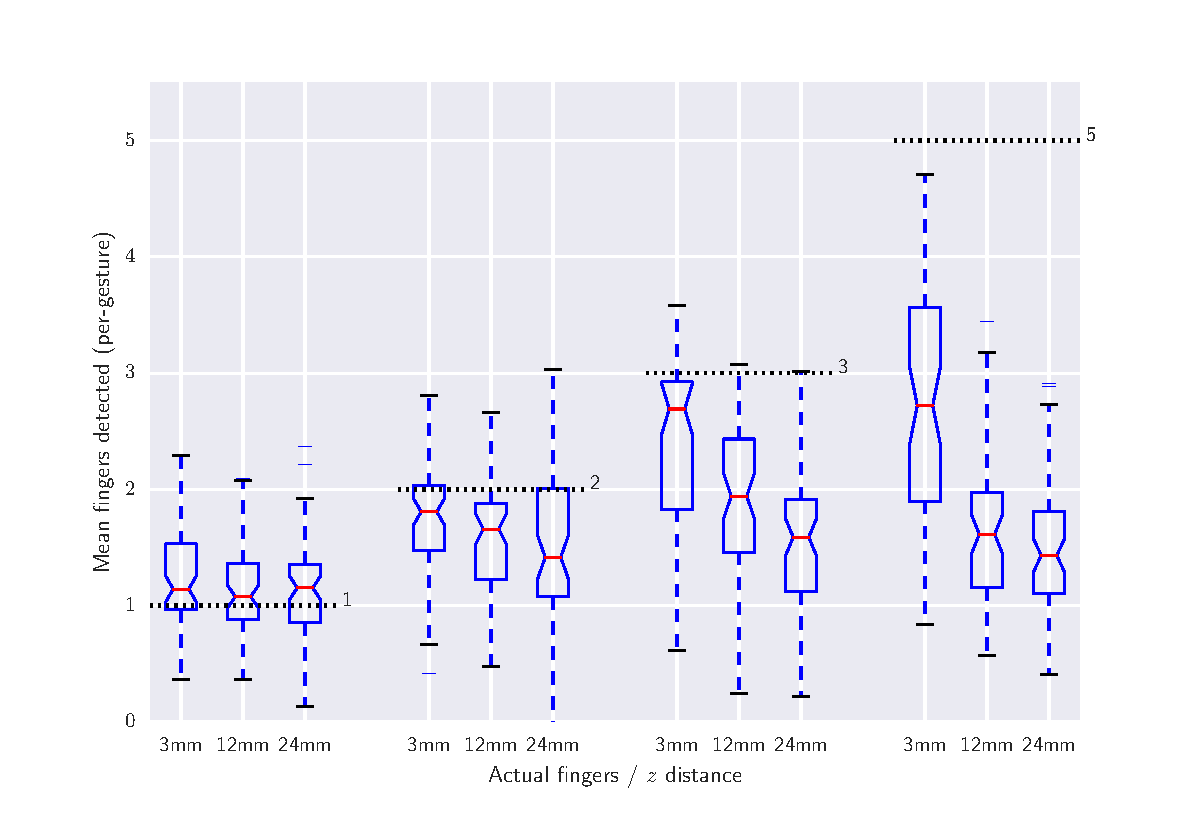
\includegraphics[width=1.0\linewidth]{images/boxplot_finger_distance.pdf}

%     \caption{Average number of fingers detected by the touch sensor at different heights above the surface, averaged over all gestures. Dashed lines indicate
%     the true number of fingers present. The Box plots include bootstrapped uncertainty notches for the median. It is clear that the device is biased toward
%     undercounting fingers, particularly at higher $z$ distances.
%     }

%     % use the notation fig:name to cross reference a figure
%     \label{fig:boxplot}
% \end{figure}

\section*{Summary}

%=============================================================================
% CONCLUSION
% Summarise the whole project for a lazy reader who didn't read the rest (e.g. a prize-awarding committee).

% ## Guidance

% -   Summarise briefly and fairly.

% -   You should be addressing the general problem you introduced in the
%     Introduction.

% -   Include summary of concrete results (“the new compiler ran 2x
%     faster”)

% -   Indicate what future work could be done, but remember: **you won’t
%     get credit for things you haven’t done**.

\chapter{Conclusion}

\section{Summary}

\section{Reflection}
% How this experience was found

\section{Side Projects}

\section{Future Work}


%=============================================================================
%
%
%=============================================================================
% APPENDICES

% Typical inclusions in the appendices are:

% -   Copies of ethics approvals (required if obtained)

% -   Copies of questionnaires etc. used to gather data from subjects.

% -   Extensive tables or figures that are too bulky to fit in the main
%     body of the report, particularly ones that are repetitive and
%     summarised in the body.

% -   Outline of the source code (e.g. directory structure), or other
%     architecture documentation like class diagrams.

% -   User manuals, and any guides to starting/running the software.

% **Don’t include your source code in the appendices**. It will be
% submitted separately.

\begin{appendices}

\chapter{First Appendix}

\loremlines{20}

\chapter{Second Appendix}

\loremlines{20}


\end{appendices}

%=============================================================================
% BIBLIOGRAPHY

% The bibliography style is abbrvnat
% The bibliography always appears last, after the appendices.
\renewcommand{\bibsection}{\chapter*{\bibname}}

\bibliographystyle{abbrvnat}

\bibliography{l4proj}

\end{document}
